\subsection{Structure du projet}

Notre projet s'organise naturellement autour d'un \it{Classifieur}. Ce dernier a besoin de pouvoir entraîner un modèle sur des données, puis de pouvoir prédire les espèces de nouvelles données, ainsi que d'évaluer les performances sur un jeu de données. Finalement, on demande au classifieur de pouvoir rechercher les meilleurs hyperparamètres pour nos données. On a ensuite des spécifications pour chacune des méthodes utilisées\\

Pour la recherche d'hyperparamètres (qui se fait sur une grille de paramètres), on a besoin d'un conteneur contenant nos paramètres et leurs domaines de recherche, permettant d'obtenir cette grille.\\

Finalement, on utilise un \it{Gestionnaire de données} pour pouvoir stocker nos jeux de données, et pour pouvoir séparer nos données en jeux d'entraînement et de validation, pour le bien des validations croisées que nous allons effectuer.\\

Notre architecture se résume ainsi sur le diagramme de classe de la \autoref{fig:class_diagram}.

\begin{figure}[h]
    \centering
    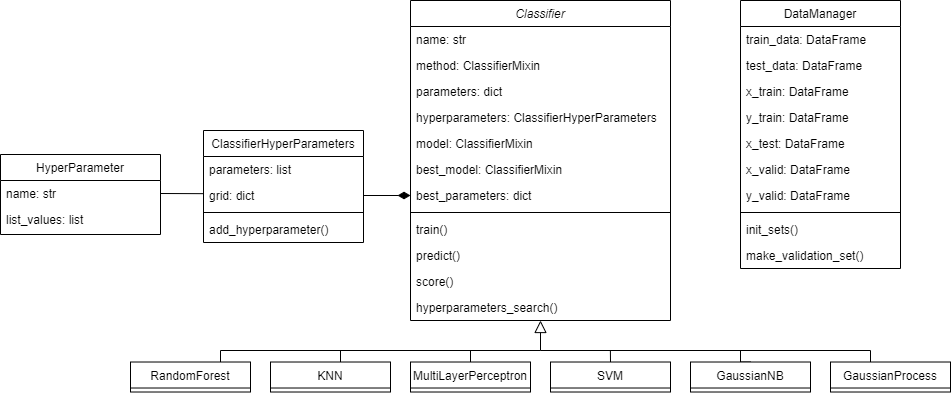
\includegraphics[scale=0.48]{Images/graphiques/class_diagram.png}
    \caption{\it{Diagramme de classes du projet}}
    \label{fig:class_diagram}
\end{figure}